\clearpage
\section{Methodik}
In diesem Kapitel werden die Analysewerkzeuge und Messverfahren vorgestellt, die in dieser Arbeit genutzt wurden. Es wurden Wetterdaten gezogen, was einer Monte-Carlo-Simulation entspricht. Sinnvolle Simulationsergebnisse wurden durch eine Pareto-Optimierung ausgewählt. Die Messung des Energiebedarfs des Antriebs wurde mittels Shunt und Datenlogger durchgeführt, die des Werkzeugs durch manuelles Auslesen eines Netzgerätes.
\subsection{Monte-Carlo-Simulation auf Solardaten}
Diese Arbeit basiert auf einer Monte-Carlo-Simulation. Dabei werden aus einem Set zufällig Samples gezogen und der Simulationscode wiederholt auf die Samples angewendet. Aus den statistischen Ergebnisse können anschließend Schlussfolgerungen gezogen werden. Das Set, aus dem gezogen wird, sind zehn Jahre an Solarstrahlungsdaten. Aus diesem Set werden kürzere Zeitreihen gezogen und in die Simulation des Energiesystems gegeben. \\
Dabei werden innerhalb eines Simulationsdurchlaufs nur Daten aus einem fest ausgewählten Zeitraum im Jahr verwendet. Dieser Zeitraum entspricht häufig einem Monat, sodass beispielsweise der Mittelwert nur über diesen Monat genommen wird wodurch saisonale Unterschiede gut dargestellt werden können. Der Monat ist damit ein \textbf{fester Parameter} in der Simulation. Die Länge der gezogenen Zeitreihe innerhalb eines Monats ist vorerst ebenfalls ein fester Parameter und entspricht dem Tankintervall. Die simulierten \textbf{Zustandsvariablen} sind der prozentuale Füllstand der Batterie und des Wasserstofftanks. Die Zustandsvariablen werden mit jedem Iterationsschritt durch sich selbst und alle anderen parameter aktualisiert. Dann wird aufgrund von Momentan- und Vergangenheitwerten heuristisch Entscheidungen getroffen. Zukünftige Information, die beispielsweise ein Wetterbericht liefern könnte, werden nicht berücksichtigt, da dies zusätzliche Simulationseingaben und einstellbare feste Parameter in die Simulation bringen würde, was den Rahmen dieser Arbeit sprengen würde.

Die \textbf{Optimierungsvariabeln} in der Simulation sind die Kapazität des Batteriespeichers in kWh, die Kapazität des Wasserstofftanks in kWh und die Fläche der Solarzelle in $m^{2}$. Weitere feste Parameter sind die Energiedichten, Wirkungsgrade und die maximale und minimale Leistung der simulierten Systembestandteile. Alle Parameter und die entsprechenden Annahmen sind unter Abschnitt \ref{simulationsparam} aufgeführt.
\subsection{Messung Energiebedarf}
Der Zeitreihe der Solardaten steht eine Zeitreihe des Energieverbrauchs gegenüber. Dafür wurden zwei Zeitreihen zusammengefügt. Der Energieverbrauch umfasst den Antrieb der mobilen Plattform DAVEGI mobile sowie die Roboterarme, die auch als Werkzeug bezeichnet werden.
\subsubsection{Messung des Antriebs}
Mit dem aktuellen Feldroboter DAVEGI mobile von Ai.Land wurde eine Testfahrt durchgeführt. Momentan wird dieser rein batterieelektrisch mit 48 V betrieben. Um die Leistung gemäß $P = U \cdot I$ zu bestimmen, haben wir mittels eines Shunts eine Zeitreihe des Stroms aufgenommen. Ein Shunt ist ein niederohmiger Widerstand, der in Reihe zur Last geschaltet ist. An diesem fällt eine geringe Spannung ab. Da der Widerstand bekannt ist, lässt sich daraus der Strom mit $U = R \cdot I$ berechnen.
Der verbaute Shunt hatte bereits ein Spannungsmessgerät mit serieller Schnittstelle integriert, sodass dieser nur an den seriellen Ausgang des Bordcomputers (NVIDIA Jetson Orin) angeschlossen werden musste. Dies wurde von einem Kollegen mit meiner Assistenz durchgeführt. Da an die serielle Schnittstelle des Orins ebenfalls der Motorregler angeschlossen ist, musste jedoch eine Sternverbindung zwischen Orin, Shunt und Motorregler hergestellt werden, sodass alle drei am gleichen CAN-Bus anliegen. Da sowohl der Motorregler als auch der Orin terminiert sind, musste darauf geachtet werden, dass beide an den Extrempunkten der Kabel anliegen. Termination bezeichnet das Einfügen eines Widerstands zwischen Signal und Masse, damit reflektierte Signale sich abbauen können. Messbereit wurde der Feldroboter dann über verschiedene Untergründe gefahren. Geteerte Feldwege, ein schlammiges Weizenfeld und ein schlammiges, abgeerntetes Maisfeld.
\subsubsection{Messung des Werkzeugs}
Als Werkzeug wird auf dem Feldroboter ein halbhumanoider Roboter montiert, d. h. nur Torso, Arme und Hände. Auch dieser hat einen Stromverbrauch. Aufgrund des anstehenden Urlaubs der bedienenden Person wurde die Leistung nicht professionell mittels Shunt ermittelt, sondern möglichst schnell durch die Videoaufnahme eines Netzgerätes. Aus diesem Video wurden mit Unterstützung eines kleinen Python-Programms alle drei Frames Strom und Spannung herausgeschrieben. Während der Datenaufnahme habe ich einen Arm des Roboters möglichst stark bewegt. Der andere Arm hat die Bewegungen synchron ausgeführt.
\subsection{Pareto-Optimierung}
Als Simulationsergebnis gibt es für jeden Monat und Tankintervall eine gemittelte Auslastung des Roboters über die Zeitreihen sowie ein Gewicht der Energieversorgung, abhängig von den drei Zustandsvariablen. 
Zusammen kann jeder Punkt im Ergebnissvektor dann als ein fünfdimensionaler Vektor aufgefasst werden, dessen Dimensionen Gewicht, Auslastung, PV-Fläche, Batteriekapazität und Tankkapazität sind. 
Plottet man die Auslastung gegen das Gewicht, so entsteht eine Punktwolke möglicher Kombinationen von Zustandsvariablen im Auslastungs-Gewicht-Raum. Viele dieser Punkte werden von anderen Punkten in beiden zu optimierenden Parametern dominiert, weshalb sie keiner sinnvollen Kombination von Zustandsvariablen entsprechen. Diese Punkte müssen entfernt werden. Dies kann durch Pareto-Optimierung erfolgen. Aus der Pareto-Optimierung folgt die Pareto-Front, die alle sinnvollen Punkte enthält.
Ein Punkt ist nicht sinnvoll, wenn er in beiden zu optimierenden Variablen von einem anderen Punkt dominiert wird. 
Ein Punkt ist sinnvoll, wenn er alle Punkte, die ihn in einer zu optimierenden Variablen dominieren, in der anderen zu optimierenden Variablen dominiert. Dies ist in Abbildung \ref{fig:Pareto-Optimierung} dargestellt. Die Pareto-Optimierung ist die einzige Methode, die die Relevanz der zu optimierenden Größe nicht bewertet. So könnte beispielsweise eine zu maximierende Funktion aus den Optimierungsgrößen erstellt werden, wobei jedoch eine Gewichtung der Größen festgelegt werden muss. Eine weitere Möglichkeit ist die sogenannte $\epsilon$-Constraint-Methode, bei der eine Optimierungsgröße als Hauptziel ausgewählt wird und alle anderen Optimierungsgrößen als Nebenbedingungen formuliert werden. Beides bringt Subjektivität in die Betrachtung ein und wird deshalb nicht verwendet. Es gibt unterschiedliche Möglichkeiten die Pareto-Optimierung zu formulieren. Gegeben ist der Ergebnisvektor, dessen Dimensionen $\mathbf{a}$ und $\mathbf{b}$ den zu optimierenden Größen entsprechen:
\begin{equation}
\mathbf{a} = [a_1, a_2, \dots, a_n], \quad
\mathbf{b} = [b_1, b_2, \dots, b_n].
\end{equation}
Für jeden Punkt $(a_i, b_i)$ wird folgende Logik ausgeführt:
Durch den Vektor $\mathbf{a}$ wird iteriert, sodass ein Vektor $\mathbf{k}$ mit Komponenten $k_i$ entsteht:
\begin{equation}
k_i =
\begin{cases}
1, & \text{falls } a_i \leq a_j, \\[1ex]
0, & \text{sonst.}
\end{cases}
\end{equation}
Der Vektor \(\mathbf{k}\) enthält Einsen überall dort, wo der Punkt \((a_i, b_i)\) von allen anderen Punkten aus \(\mathbf{a}\) dominiert wird.  
Durch elementweise Multiplikation mit \(\mathbf{b}\) entsteht der modifizierte Vektor \(\tilde{\mathbf{b}}\), der nur noch die Punkte enthält, bei denen \(a_i\) dominiert wird:
\begin{equation}
\tilde{\mathbf{b}} = \mathbf{b} \odot \mathbf{k},
\end{equation}
Um ein Pareto-Optimum zu sein, muss an den Punkten, wo \(a_i\) von allen anderen Punkten aus \(\mathbf{a}\) dominiert wird, \(b_i\) alle entsprechenden Punkte aus \(\tilde{\mathbf{b}}\) dominieren:
\begin{equation}
(a_i, b_i) \text{ ist Pareto-Optimal} \iff b_i > \max(\tilde{\mathbf{b}}),
\end{equation}



\begin{figure}
    \centering
    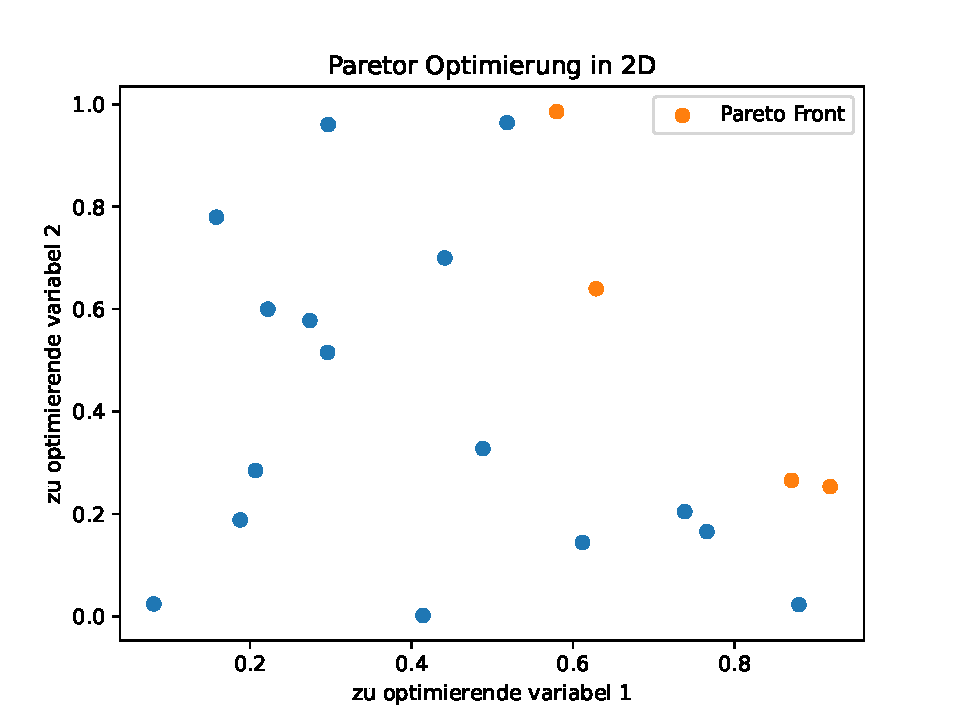
\includegraphics[width=0.6\linewidth]{Bilder/pareto-optimierung.pdf}
    \caption{Set an Punkten mit Pareto front. Alle Punkte werden von einem Punkt der Pareto-front dominiert, sodass diese die einzig sinnvollen Punkte darstellen.}
    \label{fig:Pareto-Optimierung}
\end{figure}

%\subsection{Integralerhaltende Dateninterpolation}





















\subsection{Simulationsparameter} \label{simulationsparam}
In diesem Abschnitt werden alle festen Parameter sowie ihre Werte beschrieben. Eine Veränderung dieser Parameter führt zu Änderungen im Simulationsergebnis, weshalb sie sorgfältig ausgewählt wurden.
\subsubsection{Systemkomponenten}
Es folgen die frei verkäuflichen Systemkomponenten, deren Parameter in die Simulation eingehen.
\paragraph{Photovoltaik}
Ein Standard-PV-Modul mit Glasabdeckung wiegt bei einer Größe von 2 m² üblicherweise über 20 kg. Da unter Umständen mehrere dieser Module benötigt werden, ist dies zu schwer. Deshalb wurde die Simulation mit Ultra-Leicht-Modulen durchgeführt.
Die festen Parameter wurden dem Datenblatt des PV-Moduls SMF520J-12X12UW von SUNMAN-ENERGY \cite{Sunman-PVmodule} entnommen. \\

Das PV-Modul ist ein Halbzellen-Mono-Kristallines-Silizium-Modul mit 520 Watt Peak. Es ist glasfrei und wiegt nur 7,2 kg. Es ist das erste glasfreie Modul, welches die gleichen Haltbarkeitstests wie konventionelle Glasmodule bestanden hat \cite{Sunman-PVmodule}. Die Parameter die in die Simulation eingegangen sind sind in Tabelle \ref{tab:pvparam} dargestellt. 

\begin{table}[h]
\centering
\begin{tabular}{|l|l|}
\hline
\textbf{Parameter} & \textbf{Wert} \\ \hline
Wirkungsgrad & 19.34\,\% \\ \hline
Fläche & $n \cdot 2.688\,\mathrm{m^2}$, \quad $n \in \{0,1,2,3\}$ \\ \hline
Flächengewicht & 2.679\,kg/m$^2$ \\ \hline
\end{tabular}
\caption{Paramter des PV-Moduls \cite{Sunman-PVmodule}}
\label{tab:pvparam}
\end{table}

Die offene Zellspannung beträgt 49,54 V bei einer Einstrahlung von 1000 W/m², die Spannung am Maximum Power Point beträgt 42,26 V bei einer Einstrahlung von 1000 W/m² \cite{Sunman-PVmodule}.  Deshalb bietet sich eine Parallelschaltung der Solarmodule an, damit kein DC-Wandler vor dem Laderegler nötig ist, da die Batterie in Zukunft mit 24 bis 48 Volt betrieben wird. 

\paragraph{Unterkonstruktion}
Für die PV-Module wurden Pauschalgewichte für die Unterkonstruktion veranschlagt. Veranschlagt wurden sechs Meter Aluprofile für den senkrechten Aufbau und ein Meter Aluprofile pro Quadratmeter PV-Fläche. Als Aluprofil wurde die leichteste Montageschiene von Venturama gewählt. Die PV-Montageschiene Typ 1 Standard (1,3 mm) mit dem Aluprofil 40 x 40 geht mit folgenden Parametern in die Simulation ein: 

\begin{table}[h]
\centering
\begin{tabular}{|l|l|}
\hline
\textbf{Parameter} & \textbf{Wert} \\ \hline
Unterkonstruktionsgewicht & $A \cdot 0.765 + 6 \cdot 0.765\, kg $ \\ \hline
\end{tabular}
\caption{Parameter der Unterkonstruktion \cite{Unterkonstruktion}}
\end{table}

\paragraph{Brennstoffzelle}
Für die Last wurde konservativ eine Dauerlast von ca. 450 W angenommen. In der Nacht muss die Brennstoffzelle die Last gegebenenfalls komplett allein liefern. Deshalb muss die Leistung der Brennstoffzelle mindestens 450 W betragen. 500 W würden prinzipiell reichen, allerdings ist eine 1000-W-Brennstoffzelle kaum schwerer und da der Wirkungsgrad von Brennstoffzellen bei geringeren Stromdichten höher ist, ist eine 1000-W-Brennstoffzelle effizienter. Da der Fokus dieser Arbeit auf maximaler Ausdauer und weniger auf den Kosten liegt, wird in die Simulation eine 1000-W-Brennstoffzelle einbezogen. \\

Das Produkt ist die H-1000 von Horizon Educational. In deren Produktkatalog \cite{FC-katalog} ist eine U-I-Kurve angegeben, aus der sich der Wirkungsgrad in Abhängigkeit zur Leistung bestimmen lässt. Wasser hat eine Standardbildungsenthalpie von -285,83 kJ/mol flüssig und -241,826 kJ/mol gasförmig. Beide Werte gelten bei 0 °C und 1000 hPa. Der erste Wert wird als Brennwert, der zweite als Heizwert bezeichnet. Diese Energie wird frei, wenn $H_2$ und $O_2$ zu $H_2 O$ reagieren. Da $P = U \cdot I$ ist und $I$ für die Reaktion eine Konstante ist, ist die Leistung der Reaktion direkt proportional zur Spannung. Das bedeutet, dass sich aus der Standardbildungsenthalpie direkt die Spannung berechnen lässt, die maximal zur Verfügung stehen sollte, wenn die gesamte Enthalpie in nutzbare Spannung umgesetzt wird. Dies ist aufgrund der Entropie nicht möglich. Da wir jedoch den Wirkungsgrad bestimmen möchten, muss die Spannung der Enthalpie und nicht der Gibbs-Energie verwendet werden. Diese Proportionalität wird durch die Faraday-Konstante ausgedrückt. % Es gilt Gleichung \ref{eq:prop}. 
\begin{equation} \label{eq:prop}
    U = - \frac{\Delta H}{z \cdot F}
\end{equation}
Dabei bezeichnet z in Gleichung \ref{eq:prop} die Anzahl der Elektronen pro Reaktion und F die Faraday-Konstante.
Für die Knallgasreaktion ist z = 2 und die Faraday-Konstante beträgt 96485,3321233100184 C/kmol. 
Damit ergibt sich für die enthalpische Zellspannung 1,253 Volt für den Heizwert und 1,481 Volt bezogen auf den Brennwert. In der Simulation wird immer mit dem Heizwert gerechnet, weshalb 1,253 Volt als enthalpische Spannung verwendet wird. Die UI-Kurve der Brennstoffzelle wurde mit einem Python-Script digitalisiert, sodass zwei Arrays vorlagen. 
Wird $U \cdot I$ gerechnet, so ergibt sich der Leistungs-Array, der als X-Achse verwendet wird.
Um auf der Y-Achse den Wirkungsgrad zu erhalten, wird die Spannung durch die enthalpische Spannung und die Zellzahl N geteilt. Daraus ergeben sich die Wirkungsgrad-Kurven in Abbildung \ref{fig:FC-Wirkungsgrade}.
\begin{equation}
    \eta =  \frac{U_{real}}{U_{enthalp} \cdot N}
\end{equation}
\begin{figure}
    \centering
    
\includegraphics[width=0.8\linewidth]{efficiency.pdf}
    \caption{Effizienz von zwei Brennstoffzellen in Abhängigkeit von der Leistung. Die 1000W Brennstoffzelle schlägt die 500W Brennstoffzelle aufgrund der geringeren Stromdichte}
    \label{fig:FC-Wirkungsgrade}
\end{figure}

Die Wirkungsgradkurve der 1.000-W-Brennstoffzelle wird mit einer Auflösung von einem Watt in die Simulation eingegeben. Es konnten keine Werte für eine steuerungsbedingte Minimalleistung ermittelt werden. In die Simulation fließen folgende Parameter der Brennstoffzelle ein: 

\begin{table}[h]
\centering
\begin{tabular}{|l|l|}
\hline
\textbf{Parameter} & \textbf{Wert} \\ \hline
Gewicht & 4.4 kg \\ \hline
Min. Leistung & 0.0 W \\ \hline
Max. Leistung & 1000 W \\ \hline
\end{tabular}
\caption{Paramter der Brennstoffzelle \cite{FC-katalog}}
\end{table}

\paragraph{Wasserstofftank}
Da der Wasserstofftank so leicht wie möglich sein muss, kommen nur carbonverstärkte Speicher infrage. Spectronik bietet kleine, leichte Wasserstofftanks in Größen zwischen 5 und 20 l an. Diese sind mit 350 bar angegeben. Mithilfe der idealen Gasgleichung lässt sich der Heizwert über das Volumen und den Druck bestimmen. Dieser beträgt 16 kWh für einen 20-Liter-Tank. Als Simulationsgrenzen wurden vier der 20-Liter-Tanks festgelegt. Für unterschiedliche Tankgrößen wurde die Energiedichte berechnet und ein Mittelwert gebildet. Die Parameter, die vom Wasserstofftank in die Simulation eingehen, sind: 

\begin{table}[h]
\centering
\begin{tabular}{|l|l|}
\hline
\textbf{Parameter} & \textbf{Wert} \\ \hline
Kapazität & $ n \in \{0,1,2,\dots,64\}$ kWh \\ \hline
Energiedichte & 2.2 kWh/kg \\ \hline
\end{tabular}
\caption{Parameter des Wasserstofftanks \cite{TankH2}}
\end{table}

\paragraph{Batterie und Laderegler}
Cobalt-Mangan-Lithium-Ionen-Batterien würden sich als Batterie ideal erweisen, wenn man nur auf die Energiedichte schaut. Da Lithium-Eisen-Phosphat-Batterien ($LiFePO_4$) jedoch eine längere Lebensdauer aufweisen, günstiger sind, kein Kobalt enthalten und damit die Umwelt weniger belasten, ethisch weniger fragwürdig sind und eine niedrigere Brandgefahr haben, wurde sich in der Simulation für $LiFePO_4$-Batterien entschieden, auch wenn diese eine geringere Energiedichte haben. $LiFePO_4$-Batterien gibt es in allen möglichen Größen zu kaufen. Ausgewählt wurden die Daten von LiFePO4 EVE MB31 \cite{battery}. Diese Batterie ist kostengünstig und weit verbreitet.
\begin{table}[h]
\centering
\begin{tabular}{|l|l|}
\hline
\textbf{Parameter} & \textbf{Wert} \\ \hline
Kapazität & $ n \in \{0,1,2,\dots,10\}$ kWh \\ \hline
Energiedichte & 160 Wh/kg \\ \hline
Gewicht Laderegler & 0.65 kg \\ \hline
Wirkungsgrad & 0.9 \\ \hline
\end{tabular}
\caption{Parameter der Batteriezellen und des Laderegler \cite{battery,laderegler}}
\end{table}

Außerdem wird ein Laderegler benötigt. Dafür wird der BlueSolar MPPT von Victron verwendet \cite{laderegler}. Es sei angemerkt, dass dieser die maximale Ladeleistung nur mit einem 48-V-Batteriesystem erreichen kann. In die Simulation geht nur das Gewicht ein. Es wird ein konstanter Wirkungsgrad von 0,9 beim Laden und Entladen angenommen. Dabei sind der Innenwiderstand der Batterie und der Stromverbrauch des Ladereglers berücksichtigt. Dies ist ein Schätzwert. In der Realität ist der Wirkungsgrad nicht konstant. Der Laderegler verfügt über MPP-Tracking-Fähigkeit. Es wurden nicht mehr als 8 kWh Batteriekapazität simuliert, da das Gewicht der Batterien bei 8 kWh bereits über 50 kg beträgt.


\subsubsection{Regelung und Simulationsstruktur}

\begin{wrapfigure}{l}{0.55\textwidth} % l = links, Breite = 55% der Textbreite
    \centering
    \begin{tikzpicture}[node distance=2cm, every node/.style={font=\tiny}]

    % === Nodes ===
    \node (start) [startstop] {Schleife über Zeitreihendaten (PV-Erzeugung, Last)};
    \node (residuallast) [process, below=0.3cm of start] {Residuallast = Last - PV Erzeugung};
    \node (bat_leer) [decision, below=0.3cm of residuallast] {Batterie leer?};
    \node (device_off) [process, left=1cm of bat_leer] {Gerät aus};
    \node (bat_pv) [process, below=1cm of device_off,  text width=1cm] {Batterie von PV laden};
    \node (fc_on) [decision, below=0.3cm of bat_leer, xshift=1cm] {FC eingeschaltet?};
    \node (tank_leer) [process, below=0.3cm of fc_on, xshift=-1cm] {H2 Tank leert sich};
    \node (fc_leistung) [process, below=0.3cm of tank_leer, text width=2cm, align=center] 
    {Leistungsdifferenz = Residuallast - FC Leistung};
    \node (fc_leistung2) [process, below=1.5cm of fc_on, xshift=2cm, text width=2cm, align=center] 
    {Leistungsdifferenz = Residuallast};

    \node (diff_pos) [decision, below=2.5cm of fc_on] {Leistungsdifferenz > 0?};

    \node (bat_entladen) [process, below=0.3cm of diff_pos, xshift=1.2cm] {Batterie entladen};
    \node (bat_laden) [process, below=0.3cm of diff_pos, xshift=-1.2cm] {Batterie laden};

    \node (pv_module) [decision, below=1cm of diff_pos] {PV Module vorhanden?};

    \node (nacht) [decision, below=0.3cm of pv_module, xshift=1cm] {Nachtbetrieb?};

    \node (nachtregelung) [process, below=2cm of pv_module] {FC Nachtregelung};
    \node (reinH2) [process, left=0.3cm of nachtregelung, text width=2cm, align=center]{FC Regelung für reinen H2 Betrieb};
    \node (tagregelung) [process, right=0.3cm of nachtregelung]{FC Tagesregelung};

    \node (zustand) [process, below=12.5cm of bat_leer]{Zustandsparameter aktualisieren};
    \node (zeitschritt) [startstop, below=0.3cm of zustand]{Nächster Zeitschritt};

    \node (text) [textnode, below=0.2cm of bat_entladen, xshift=1.5cm] {FC Leistungsregelung};

    % === Connections ===
    \draw [arrow] (start) -- (residuallast);
    \draw [arrow] (residuallast) -- (bat_leer);

    \draw [arrow] (bat_leer.west) -- (device_off.east) node[midway, above] {ja};
    \draw [arrow] (bat_leer.south) -| (fc_on.north) node[midway, above] {nein};
    \draw [arrow] (device_off.south) -- (bat_pv.north);
    \draw [arrow] (bat_pv.south) |- (zustand.west);

    \draw [arrow] (fc_on.south) -| (tank_leer.north) node[midway, above] {ja};
    \draw [arrow] (fc_on.south) -| (fc_leistung2.north) node[midway, above] {nein};
    \draw [arrow] (tank_leer.south) -- (fc_leistung.north);

    \draw [arrow] (fc_leistung.south) -- (diff_pos);
    \draw [arrow] (fc_leistung2.south) -- (diff_pos);

    \draw [arrow]  (diff_pos.south) -| (bat_entladen.north) node[midway, above] {nein};
    \draw [arrow]  (diff_pos.south) -| (bat_laden.north) node[midway, above] {ja};

    \draw [arrow] (bat_entladen.south) -- (pv_module);
    \draw [arrow] (bat_laden.south) -- (pv_module);

    \draw [arrow]  (pv_module.south) -| (reinH2.north) node[midway, above] {nein};
    \draw [arrow]  (pv_module.south) -| (nacht.north) node[midway, above] {ja};

    \draw [arrow]  (nacht.south) -| (tagregelung.north) node[midway, above] {nein};
    \draw [arrow]  (nacht.south) -| (nachtregelung.north) node[midway, above] {ja};

    \draw [arrow] (tagregelung) -- (zustand);
    \draw [arrow] (nachtregelung) -- (zustand);
    \draw [arrow] (reinH2) -- (zustand);

    \draw [arrow] (zustand) -- (zeitschritt);


    === Background for Subgraph ===
    \begin{pgfonlayer}{background}
    \node[fill=gray!20,fit=(pv_module) (reinH2) (nacht) (tagregelung) (nachtregelung) (text),rounded corners,inner sep=0.1cm]{};
    \end{pgfonlayer}

    \end{tikzpicture}
    \caption{Flowchart der Simulation}
    \label{fig:flowchart}
\end{wrapfigure}

Im Abschnitt „Stand der Technik” wurde eine Regelung mittels modellprädiktiver Kontrolle (MPC) vorgeschlagen. Dies wäre in einer Simulation gut umzusetzen, da die historischen Solardaten vorliegen. In einem Roboter ist eine solche Regelung eine technische Herausforderung, da dieser sich regelmäßig mit dem Internet verbinden müsste, um Wettervorhersagen abzurufen. Dies ist insbesondere bei einem Feldroboter, der unter Umständen auf entlegenen Feldern eingesetzt wird, schwer umzusetzen. Deshalb, und weil zum Zweck der Auslegung des Energiesystems keine kompliziertere Regelung benötigt wird, wird eine Regelung verwendet, die nur die lokal auf dem Roboter vorliegenden Daten berücksichtigt. Dies ist dann ein State-Feedback-Controller. Dieser wird aufgrund des Fehlens relevanter Informationen nicht so optimal sein wie eine MPC mit Wettervorhersage, sollte aber für eine Auslegung der Komponenten des Energiesystems ausreichen. \\

In Abbildung \ref{fig:flowchart} ist die innerste Schleife des Simulationscodes zusammenfassend dargestellt. In dieser Schleife wird über die Zeit iteriert, wodurch die Zeitreihen der PV-Erzeugung und des Energiebedarfs des Roboters (Last) berücksichtigt werden. Zunächst wird die Residuallast berechnet, die sich aus der Last minus der PV-Erzeugung ergibt. Das bedeutet, dass, wenn PV-Erzeugung vorhanden ist, die Last des Roboters zuerst bedient wird, ohne Umwege über die Batterie. Ist die Batterie jedoch leer, d. h. liegt der Ladezustand unter einem Schwellwert von 5 \%, wird der Roboter ausgeschaltet und der PV-Strom zum Aufladen der Batterie verwendet. Ist die Brennstoffzelle aktiv, wird die Leistung der Brennstoffzelle von der Residuallast abgezogen. Ist die verbleibende Last (Leistungsdifferenz) größer als Null, muss die Batterie unterstützen. Im gegenteiligen Fall wird sie geladen. Im grau hinterlegten Abschnitt von Abbildung \ref{fig:flowchart} wird die Leistungsregelung vereinfacht dargestellt. Hier wird die Leistung der Brennstoffzelle (FC) so geregelt, dass ein möglichst ausdauernder Betrieb mit hohem Wirkungsgrad möglich ist. In der Simulation wird bei der Regelung der Brennstoffzellenleistung grundlegend zwischen reinem Wasserstoffbetrieb, Tag- und Nachtregelung unterschieden. 

\subsubsection{FC Leistungsregelung am Tag}
Im Tagbetrieb schaltet sich die Brennstoffzelle nur ein, wenn die Batterie einen prozentualen Schwellwert unterschreitet. Die Leistung der Brennstoffzelle wird dann aus dem gleitenden Durchschnitt der letzten zehn Minuten Residuallast gebildet. Die Residuallast ist die Last minus der von den PV-Modulen bereitgestellten Leistung. Ändert sich die angeforderte Leistung an die Brennstoffzelle, so wird dieser Wert nicht sofort eingestellt, sondern proportional über mehrere Schritte angenähert. Dies entspricht dem P-Anteil eines PID-Reglers. Dadurch wird ein glattes Hoch- und Runterfahren der Brennstoffzelle erreicht, auch bei stark schwankender Residuallast. Dadurch deckt die Brennstoffzelle die Grundlast, allerdings keine Spitzenlast bzw. hochfrequente Anteile. Die hochfrequenten Anteile werden von der Batterie abgedeckt. \\

\subsubsection{FC Leistungsregelung in der Nacht}
Der Nachtbetrieb ist grundsätzlich verschieden. Zwar wäre es möglich, die gleiche einfache Logik wie am Tag umzusetzen, dies würde jedoch zu einem seriellen Betrieb von Batterie und Brennstoffzelle führen, was weniger effizient ist als ein Parallelbetrieb beider Energiequellen. 
Im Tagesbetrieb ist ein Parallelbetrieb jedoch nicht sinnvoll, da die Batterie ohne Wettervorhersage sonst nicht als Speicher für PV-Strom genutzt werden kann. Für den Nachtbetrieb muss die Zeit des Nachtbetriebs festgelegt werden. Dies geschieht anhand der historischen Solardaten. Wenn die Leistung für zehn Iterationsschritte unter 10 W fällt und danach für zehn Iterationsschritte größer als 10 W ist, wird dies als Zeitpunkt des Sonnenaufgangs gewertet. Am Abend wird der Zeitpunkt des Sonnenuntergangs entsprechend umgekehrt ermittelt. Nach spätestens 24 Stunden Tagbetrieb ist damit das Zeitfenster für die folgende Nacht festgelegt. Dieses Zeitfenster wird abends und morgens noch um je eine Stunde verlängert. Das Ziel besteht darin, in der Nacht Brennstoffzelle und Batterie parallel zu betreiben, sodass am nächsten Morgen möglichst exakt eine einstellbare prozentuale Restmenge in der Batterie vorhanden ist. Dazu wird in jedem Iterationsschritt die Energie bestimmt, die nötig ist, um den Feldroboter bis zum Ende der Nacht zu betreiben. Von dieser Energie wird die Differenz des aktuellen Füllstands der Batterie und dem, was am nächsten Morgen noch in der Batterie sein soll, abgezogen. Die restliche Energie wird durch die Zeit bis zum Ende des Zeitfensters geteilt und stellt damit die angeforderte Leistung an die Brennstoffzelle dar. Dies bewirkt einen konstanten Betrieb unterhalb der Residuallast während der Nacht. Die durch die Regelung entstehende Parameter sind in Tabelle \ref{tab:paramregelung} aufgeführt. \\

\begin{table}
\centering
\begin{tabular}{|l|l|}
\hline
\textbf{Parameter} & \textbf{Wert Tagbetrieb} \\ \hline
Zeitintervall Residuallast & 5 min. \\ \hline
FC-An bei & 0.1 Füllstand-Batterie \\ \hline
FC-Aus bei & 0.2 Füllstand-Batterie \\ \hline
\textbf{Parameter} & \textbf{Wert Nachtbetrieb} \\ \hline
Zeitintervall Residuallast & 5 min. \\ \hline
Zeitfenster offset & 1 h \\ \hline
FC-An bei & 0.9 Füllstand-Batterie \\ \hline
Sonnenaufgang Restmenge & 0.3 Füllstand-Batterie \\ \hline
\end{tabular}
\caption{Parameter der Brennstofzellenregelung}
\label{tab:paramregelung}
\end{table}

Der Roboter hat eine vom Batteriefüllstand abhängige Abschalt- und Wiedereinschaltgrenze. Die Zeit, die der Roboter im Zustand „An” verbringt, wird erfasst, um die Auslastung im Zeitintervall zu bestimmen. In der Simulation sind beide Werte recht niedrig gewählt, damit sie der Batteriekapazität der Simulation entsprechen. Um die Lebensdauer der Batterien zu erhöhen, lohnt es sich, diesen Wert zu erhöhen. \\



\begin{table}
\centering
\begin{tabular}{|l|l|}
\hline
\textbf{Parameter} & \textbf{Wert Tagbetrieb} \\ \hline
Roboter-Aus bei & 0.05 Füllstand-Batterie \\ \hline
Roboter-An bei & 0.15 Füllstand-Batterie \\ \hline
\end{tabular}
\caption{Aus- und Einschaltparameter}
\end{table}

\subsubsection{FC Leistungsregelung bei reinem Wasserstoffbetrieb}
In der Simulation ist standardmäßig festgelegt, dass die Batterie ausschließlich durch Solarstrom und nicht durch Wasserstoff aufgeladen wird. Dies kann jedoch zu Problemen führen, wenn keine PV-Module verwendet werden. Für diesen Fall wird eine andere heuristische Steuerung verwendet. Ist der Füllstand der Batterie niedriger als 0,4, so wird die angeforderte Brennstoffzellenleistung pauschal um 30 W über die Residuallast erhöht. Dies lädt die Batterie langsam wieder auf. Ist der Batteriefüllstand größer als 0,5, wird die Brennstoffzellenleistung pauschal um 30 W niedriger gehalten als die Residuallast, was die Batterie entlädt. Der Batteriefüllstand pendelt sich somit auf Dauer bei ca. 50 \% ein und die Brennstoffzelle wird nahezu mit konstanter Leistung betrieben, was eine maximale Effizenz bedingt.

\subsubsection{Weitere Annahmen}
Ebenfalls wird davon ausgegangen, dass jede Zeitreihe zu einer bestimmten Uhrzeit startet. Jede Kombination von Energiesystemkomponenten, die ein bestimmtes Gewicht überschreitet, wird vorab entfernt und geht nicht in die Simulation ein. Für die Simulation wird eine Schrittweite von 60 Sekunden verwendet. Dadurch werden hochfrequente Lastspitzen in der Simulation nicht abgebildet. Deshalb wurde die Funktion, um Lade- und Entladestrom zu begrenzen, entfernt bzw. die Werte auf unendlich gesetzt. Zu prüfen ist, ob die einzusetzende Batterie die maximalen Leistungsspitzen aus der Lastmessung abdecken kann. Außerdem wird angenommen, dass das PV-Panel waagerecht montiert ist. Dadurch wird das Festlegen einer abzufahrenden Strecke, das Tracken der Sonnenstrahlen sowie das Differenzieren in Global- und Diffusstrahlung erspart. In der Realität würden die PV-Module in einer Dachform mit einem Winkel von 15 bis 35° zur Erde angebracht werden, da dies den Reinigungsaufwand deutlich reduziert.

\begin{table}[h]
\centering
\begin{tabular}{|l|l|}
\hline
\textbf{Parameter} & \textbf{Wert Tagbetrieb} \\ \hline
Start Zeit & 8 Uhr \\ \hline
Maximalgewicht & 150 kg \\ \hline
Simulationsauflösung & 60 sek. \\ \hline
\end{tabular}
\caption{Weitere paramter}
\end{table}


\subsection{CAD Modell des Feldroboters} 

Um die Grenzen der zu optimierenden Simulationsparameter auszuloten, wurde durch einen Kollegen das bestehende CAD-Modell des Feldroboters um die Hauptkomponenten des Energiesystems ergänzt. Es konnten vier 20-Liter-Wasserstofftanks untergebracht werden, von denen jeweils zwei senkrecht über der Fahrspur zwischen den Rädern hängen. Die Brennstoffzelle ist im Gehäuse untergebracht, direkt neben der Aufhängung für den Halbhumanoiden. Die Batteriepakete können ebenfalls im Gehäuse untergebracht werden. Für die PV-Module gibt es zwei mögliche Anordnungen, die in Abbildung \ref{fig:robots} zu sehen sind. Bei zwei PV-Modulen bietet sich eine Dachstruktur an. Diese bedeckt jedoch momentan die GPS-Antenne, wodurch das Signal schlecht wird. Deshalb wird bei der Option mit einem PV-Modul das Gehäuse nicht bedeckt. Das Gesamtgewicht des Feldroboters ohne Energiesystem kann auf knapp 300 kg geschätzt werden. Je nach Auslegung des Energiesystems kommen 20 bis 100 kg dazu.

\begin{figure}[hbtp]
    \centering
    % Erste Reihe
    \begin{subfigure}{0.4\textwidth}
        \centering
        
\includegraphics[width=\textwidth]{rob1.png}
        \label{fig:rob1}
    \end{subfigure}
    %\hfill
    \begin{subfigure}{0.4\textwidth}
        \centering
        
\includegraphics[width=\textwidth]{rob2.png}
        \label{fig:rob2}
    \end{subfigure}
    
    % Zweite Reihe
    \begin{subfigure}{0.4\textwidth}
        \centering
        
\includegraphics[width=\textwidth]{rob3.png}
        \label{fig:rob3}
    \end{subfigure}
    %\hfill
    \begin{subfigure}{0.4\textwidth}
        \centering
        
\includegraphics[width=\textwidth]{rob4.png}
        \label{fig:rob4}
    \end{subfigure}
    \caption{CAD Modell des Feldroboters Aplamo mit 4 20L Wasserstofftanks und 1 bzw. 2 PV-Modulen. Die Brennstoffzelle ist im Gehäuse untergebracht}
    \label{fig:robots}
\end{figure}
